\documentclass[11pt,a4paper]{article}
% Optics Express / revtex class files are not installed on this system.
% Single-column article layout, set for an Optics Express or Optics Letters design paper.
% TODO: confirm department/college, postal code, and corresponding-author e-mail.

\usepackage[margin=0.95in]{geometry}
\usepackage{times}
\usepackage{mathptmx}
\usepackage{amsmath,amssymb}
\usepackage{graphicx}
\usepackage{booktabs}
\usepackage{longtable}
\usepackage{tabularx}
\usepackage{array}
\usepackage{float}
\usepackage[numbers,sort&compress]{natbib}
\usepackage[colorlinks=true,citecolor=blue,linkcolor=blue,urlcolor=blue]{hyperref}

\graphicspath{{fig/}}
\renewcommand{\arraystretch}{1.12}
\newcolumntype{Y}{>{\raggedright\arraybackslash}X}

\title{Adaptive poling for high-purity heralded single photons on thin-film lithium niobate: a design study}

\author{%
Xinlei Chen and Yuanhua Li\thanks{Corresponding author. E-mail to be confirmed.}\\
Shanghai University of Electric Power, Shanghai, China%
}
\date{}

\begin{document}
\maketitle

\begin{abstract}
Thin-film lithium niobate can host heralded single-photon sources, but film-thickness variations distort quasi-phase matching and cut the spectral purity once the device is made long.
Adapted poling is already used to restore second-harmonic efficiency, and it has been suggested for photon-pair sources, but it has not been used to compute the heralded purity.
This design study is entirely a simulation.
On a 5~mm device whose thickness follows the measured trace of Chen \emph{et al.}, the uncompensated intensity-only purity spans only 0.38--0.82.
Reaching the 0.98 purity that Kuttner \emph{et al.}\ estimate from their phase-matching function requires thickness fluctuations about seven times smaller, an RMS of roughly 0.1--0.3~nm over 5~mm.
The Monte Carlo uses a film-thickness sensitivity of $-3.161$~rad/mm/nm for a TM pump: the difference quotient between 560 and 640~nm, an average slope over that 80~nm, not the local derivative at 600~nm.
Only that coefficient was updated.
The group-velocity ratio and the poling period in the scan are still the TE-pump values; both have to be recomputed if the device is confirmed to use a TM pump.
Uncompensated, a median purity of 0.90 is reached only at 2~mm (0.944), at a relative coincidence rate of 0.143.
Measuring every 0.2~mm reaches 5~mm (median purity 0.923, 10th--90th percentile 0.88--0.95), 2.4 times that rate.
Measuring every 0.1~mm reaches 10~mm (median 0.903, percentile 0.80--0.92), 4.5 times; the median only just clears 0.90 and the 10th percentile is 0.80, so the purity does not stay above 0.90.
Measuring every 0.04~mm also reaches 10~mm (median 0.913, percentile 0.87--0.95), again 4.5 times.
Those rates use the measured collection loss of Zhao \emph{et al.}: propagation loss $-0.54$~dB/cm near 1569~nm, facet transmission 0.200 ($-7$~dB per facet; the facets were unpolished and unoptimized, so this is a conservative case and not an intrinsic device limit), and detection efficiency 68\%, with no pump propagation loss.
The heralding efficiency is then fixed by that loss formula: 0.134 at 2~mm and 0.120 at 20~mm.
An optimistic model (0.3~dB/cm, facet transmission 0.5, detection efficiency 0.8) is only an upper bound.
It raises the heralding efficiency by about a factor of three (0.397 at 2~mm).
Under the previous coefficient, $-3.687$~rad/mm/nm (TE pump), the 0.1~mm pitch reached only 5~mm at a median purity of 0.944, 2.4 times; that result is a comparison, not the design point.
Kuttner's length, width, and etch depth are not given in the original paper.
The width noise and the thickness-measurement error used here are assumptions, and the conclusions move when they change.
There is no experiment of our own.
\end{abstract}

\section{Introduction}
A heralded photon from spontaneous parametric down-conversion is useful only to the extent that its partner fixes the quantum state.
On thin-film lithium niobate (TFLN) that requirement is a design problem: the phase-matching function has to be made separable, and it has to survive the film that is actually grown.
Kuttner \emph{et al.}\ integrated two type-II sources on x-cut TFLN and measured joint-spectral-intensity purities of 95.2\% and 93.8\%, with purities of 98.0\% and 98.3\% estimated from the phase-matching function \cite{Kuttner2026}.
The film is 600~nm thick.
The pump is TM at 764~nm and produces a TE signal and a TM idler.
The poling is a Gaussian deleted-domain profile \cite{Tambasco2016,Kuttner2026}, not a uniform grating.
In the text they note that compensating film-thickness variations by the method of Chen \emph{et al.}\ would let the phase-matched section be made longer and the bandwidth narrower.

That method, adapted poling, was demonstrated for second-harmonic generation.
Chen \emph{et al.}\ varied the local poling period with the measured film thickness, recovered the ideal length-squared scaling, and reported an efficiency of order $10^{4}$\,\%/W without a cavity \cite{Chen2024}.
Xin \emph{et al.}\ measured a wafer on a 100~\textmu m grid and used a non-periodic quasi-phase-matching grating to raise the yield of second-harmonic devices at a target wavelength \cite{Xin2025}.
Both papers treat classical conversion efficiency or wavelength yield.
Neither computes the spectral purity of a heralded photon.

The broader point, that a longer nonlinear waveguide tolerates less fabrication error, is not new.
Santandrea \emph{et al.}\ showed it for titanium-diffused lithium niobate, with width errors rather than film thickness, and they evaluated squeezing, frequency-bin encoding, and bandwidth compression \cite{Santandrea2019}.
They did not treat TFLN, film thickness, adapted poling, or the spectral purity of a heralded photon.
A two-colour TFLN source has since suggested, in one sentence, that thickness variations could be compensated by adapted poling or by changing the waveguide width along the guide \cite{Babel2025,Chen2024,He2024}.
That source is type-0 (532~nm to about 810~nm and 1550~nm), with a 3~mm poled section and an effective poling length of 2.78~mm, 93\% of the design.
The film thickness is an average of five points, $607\pm 1$~nm, with no trace along the waveguide.
The suggestion is not carried out, and the purity is not calculated.
We do not claim that adapted poling of a TFLN photon-pair source has never been discussed.
What has not been done is a quantitative map from measured thickness traces to heralded purity, length, and the metrology needed to hold a stated purity.

This paper is that map.
It is a design study.
Section~\ref{sec:model} states the model and which numbers are measured, calibrated, or assumed.
Section~\ref{sec:kuttner} asks what purity a Chen-like wafer actually gives, and what uniformity would be required to match Kuttner's result.
Section~\ref{sec:adapt} asks how far adapted poling extends the length at a fixed median purity.
Section~\ref{sec:limits} collects the limits that have to travel with the numbers.

\section{Model and parameters}
\label{sec:model}
The device follows Kuttner's type-II process: an x-cut film, a TM pump at 764~nm, a TE signal, and a TM idler, with wavelengths near 1550~nm for the generated pair \cite{Kuttner2026}.
The nominal film thickness is the stated 600~nm.
The length, the width, and the etch depth are not stated in that paper, including the supplement, which contains figures but no geometry table.
Two indirect length estimates are used only as bounds.
A chip photograph carries a 5~mm scale bar; if the chip were square the electrode region would be about 6~mm, but the photograph is oblique, so this is only ``a few millimetres.''
The pumps they prepare, 1.84~nm and 1.65~nm, are chosen to match the phase-matching bandwidth.
In our Gaussian model with width $\sigma=0.25L$, the optimal pump bandwidth is about 7.6~nm per millimetre of length.
Read as a full width at half-maximum, 1.7~nm corresponds to $L\approx 4.3$~mm; read as a $1/e^{2}$ width, it corresponds to about 7~mm.
The length used below for the comparison is therefore the interval 4--7~mm, not a single design value.
The width is read from their scanning-electron micrograph as about 0.9~\textmu m, with a reading error of about $\pm 0.2$~\textmu m, and the calculation uses 1.0~\textmu m.
The etch depth is not given.
We assume 300~nm.
These three substitutions are assumptions about their device, not measurements.

With the pump set to TM, the group-velocity ratio is $|A/B|=3.89$.
The phase-matching function is then a nearly vertical band, which matches the direction of their measured map (signal axis about 1490--1530~nm).
An earlier version of this model used a TE pump.
That assignment is wrong for this source and is not used in Sec.~\ref{sec:kuttner}.
Section~\ref{sec:adapt} uses the TM-pump thickness sensitivity, but the group-velocity ratio and the poling period in that scan are still the TE-pump values.
If the device is confirmed to use a TM pump, those two have to be recomputed.
That split is stated in Sec.~\ref{sec:adapt} and is not hidden in the caption.

Modes are computed with a semi-vectorial finite-difference solver and the Sellmeier equation of Zelmon, Small, and Jundt \cite{Zelmon1997}.
The film-thickness sensitivity of the mismatch, recomputed for the TM pump on a width of 1.4~\textmu m, is $-3.161$~rad/mm/nm.
That number is the difference quotient between 560 and 640~nm, an average slope over that 80~nm, not the local derivative at 600~nm.
The same derivative split into 560--600~nm and 600--640~nm is $-3.32$ and $-3.00$, so the slope is not linear.
The same solver, on the second-harmonic geometry of Zhao \emph{et al.}\ \cite{ZhaoLu2023}, overestimates the published thickness derivative by about 7\% for a vertical sidewall and by about 3\% for a $60^{\circ}$ sidewall.
We take a 10\% error on the thickness sensitivity as the calibration uncertainty of the tool.
A 20\% shift does not, in the check of Sec.~\ref{sec:kuttner}, move a Chen-like 5~mm device up to a purity of 0.98.
The etch-depth and width derivatives remain high, by about 36\% and 28\% at $60^{\circ}$ relative to the same paper.
The main scan uses the vertical-sidewall values for those two derivatives, which overstates their damage and is the conservative choice.
Table~\ref{tab:calib} records the comparison.
On the measured etch variation the etch term is small; the width term is set by an assumed noise, discussed below.

The poling envelope is a Gaussian deleted-domain profile with $\sigma=0.25L$ \cite{Tambasco2016}.
With no disorder, the optimal pump bandwidth and the ideal purity are given in Table~\ref{tab:ideal}.
The pump bandwidth is then frozen at that ideal value.
It is not retuned for each disordered device.
A residual pump chirp is drawn uniformly from $\pm 0.25\tau^{2}$.
That range is an assumption.
Purity is the Schmidt purity of the joint spectral amplitude.
Where the comparison is with a purity estimated from a measured phase-matching function, we instead report the intensity-only purity, which is the same kind of estimator.
An intensity measurement does not see a pump chirp, and using it as a purity overestimates the state when the correlations are in the phase \cite{Graffitti2018}.

\begin{table}[t]
\centering
\caption{Ideal Gaussian device after the pump is set to TM.
The bandwidth is the optimum for that length.
No film disorder.}
\label{tab:ideal}
\begin{tabular}{lccccc}
\toprule
Length (mm) & 1 & 2 & 3 & 5 & 7 \\
\midrule
Optimal pump bandwidth (nm) & 7.6 & 3.8 & 2.5 & 1.5 & 1.1 \\
Ideal purity & 0.993 & 0.995 & 0.995 & 0.995 & 0.995 \\
\bottomrule
\end{tabular}
\end{table}

Two published thickness traces are the disorder, not a random process drawn to match a variance.
Chen \emph{et al.}, Fig.~1d, is a 21~mm line, digitized from the vector artwork (526 points; reading error below 0.01~nm, which does not include any smoothing the authors may have applied) \cite{Chen2024}.
The thickness runs from 597.2 to 609.7~nm.
Inside a 5~mm window the RMS is 0.64--1.81~nm.
The spectral slope is $-1.44$ between 0.2 and 5~mm$^{-1}$ and $-1.90$ above 5~mm$^{-1}$, steeper than $1/f$.
Structure shorter than 0.2~mm contributes an RMS of at most 0.31~nm, and that bound can include the instrument.
It is one line on one wafer.
Xin \emph{et al.}, Fig.~2b, is a 5~mm line sampled every 100~\textmu m (51 points), read from a raster image to about $\pm 0.2$~nm \cite{Xin2025}.
The pre-etch film has RMS 0.82~nm and peak-to-peak 3.15~nm.
The etch-depth trace has RMS 0.20~nm, and that trace is what we use for etch disorder.
On Chen windows, where no etch trace was published, the etch disorder is a $1/f$ process with RMS 0.2~nm.

Table~\ref{tab:params} is the parameter list for the Monte Carlo.
Every assumed entry is marked.
Loss, coupling, and detection efficiency change the heralding efficiency and the coincidence rate.
They do not change the purity.

{\small
\setlength{\tabcolsep}{3pt}
\begin{longtable}{@{}>{\raggedright\arraybackslash}p{2.35cm}>{\raggedright\arraybackslash}p{6.15cm}>{\raggedright\arraybackslash}p{6.55cm}@{}}
\caption{Parameters of the Monte Carlo design scan.
``Assumed'' means the value is not taken from a measured number in the cited paper.
The scan uses $-3.161$~rad/mm/nm (TM pump, 560--640~nm difference quotient). The group-velocity ratio and the poling period are still the TE-pump values; see Sec.~\ref{sec:adapt}.}
\label{tab:params}\\
\toprule
Parameter & Value used & Source \\
\midrule
\endfirsthead
\multicolumn{3}{@{}l}{\tablename~\thetable\ continued}\\
\toprule
Parameter & Value used & Source \\
\midrule
\endhead
\bottomrule
\endfoot
Film-thickness trace & Chen Fig.~1d (21~mm); Xin Fig.~2b (5~mm) & Both full texts. Chen from vector paths ($<0.01$~nm). Xin from a raster ($\pm 0.2$~nm). \\
$\mathrm{d}\Delta k/\mathrm{d}t$, this device & $-3.161$~rad/mm/nm in this scan. Previous scan: $-3.687$~rad/mm/nm & This scan: TM pump, difference quotient from 560 to 640~nm (average slope over 80~nm, not the local derivative at 600~nm), width 1.4~\textmu m. Previous: TE pump, $\pm 10$~nm central difference. Solver calibrated on Ref.~\cite{ZhaoLu2023} (7\% high at $90^{\circ}$, 3\% high at $60^{\circ}$). Group-velocity ratio and poling period in the scan are still the TE-pump values. \\
Etch-depth variation & Xin's measured etch trace, RMS 0.20~nm; $1/f$ at 0.2~nm on Chen windows & Xin Fig.~2b. \\
Etch and width sensitivities & Vertical-sidewall values (high relative to Ref.~\cite{ZhaoLu2023}) & Still 36\% and 28\% high at $60^{\circ}$. Conservative. \\
Width variation & $1/f$, RMS 2~nm. Scan: 0, 2, 5, 10~nm & \textbf{Assumed.} An AFM in Ref.~\cite{ZhaoLu2023} was below their 13~nm estimate; no measured RMS is given. \\
Thickness measurement error & 0.3~nm, white. Scan: 0.3, 0.5, 1.0~nm & \textbf{Assumed.} Xin \emph{et al.}\ cite the ellipsometer and give no number. \\
Measurement pitch & 0.1~mm. Also 0.2 and 0.04~mm & 0.1~mm: Xin \cite{Xin2025}. 0.2~mm, 17~\textmu m spot: Zhao \emph{et al.}\ \cite{ZhaoLu2023}. 0.04~mm: \textbf{assumed}. \\
Residual pump chirp & Uniform on $\pm 0.25\tau^{2}$. Scan: 0, 0.25, 0.5, $1.0\tau^{2}$ & \textbf{Assumed.} \\
Pump bandwidth & Frozen at the ideal optimum & Conservative: no per-device retune. \\
Propagation loss, signal/idler & $-0.54$~dB/cm near 1569~nm (main case) & Supplemental material of Ref.~\cite{Zhao2020}, cut-back. 0.3~dB/cm is the \textbf{optimistic upper bound} only, not the main case. The ``$<1$~dB/cm'' figure was a search-excerpt paraphrase and is not quoted. \\
Pump propagation loss & None in the main case & Separate case only: $-3.21$~dB/cm near 785~nm, same supplemental, cut-back. That term changes the generation rate, not only collection. The earlier 0.6~dB/cm value was \textbf{assumed} and is not used. \\
Facet transmission, each facet & 0.200, i.e.\ $-7$~dB/facet at 1570~nm (main case) & Supplemental material of Ref.~\cite{Zhao2020}. Facets were unpolished and unoptimized, so 0.200 is a \textbf{conservative case, not an intrinsic device limit} (mode overlap accounts for $-3$~dB/facet; the rest is roughness and higher-order modes; $-15$~dB/facet at 785~nm). Transmission 0.5 is the \textbf{optimistic upper bound} only. The 4.9~dB/facet lensed-fiber figure is in Ref.~\cite{Shi2024}. \\
Detection efficiency & 68\% (main case) & Supplemental material of Ref.~\cite{Zhao2020}: about 68\% for two SNSPDs (the third was about 90\%; there is no single device-wide 68\% beyond those two). Detection efficiency 0.8 is the \textbf{optimistic upper bound} only. \\
\end{longtable}
}


\begin{table}[ht]
\centering
\caption{Sidewall check on the second-harmonic geometry of Zhao \emph{et al.}\ \cite{ZhaoLu2023}.
The published numbers are $-4.018$~\textmu m$^{-2}$, $1.842$, and $-0.485$ in the units of that paper.
Our device is not this geometry; the table only calibrates the solver.}
\label{tab:calib}
\begin{tabular}{lccc}
\toprule
Sidewall & $\partial\Delta\beta/\partial t$ & $\partial\Delta\beta/\partial h$ & $\partial\Delta\beta/\partial w$ \\
\midrule
$90^{\circ}$ & $-4.28$ & 3.60 & $-0.67$ \\
$75^{\circ}$ & $-4.22$ & 3.06 & $-0.65$ \\
$65^{\circ}$ & $-4.17$ & 2.69 & $-0.63$ \\
$60^{\circ}$ & $-4.14$ & 2.51 & $-0.62$ \\
Published \cite{ZhaoLu2023} & $-4.018$ & 1.842 & $-0.485$ \\
\bottomrule
\end{tabular}
\end{table}

\section{What a measured wafer does to the purity}
\label{sec:kuttner}
Figure~\ref{fig:thick} shows the two traces the rest of the paper uses.
The question in this section is narrow: if a device of Kuttner's length sat on a film as uneven as Chen's, what purity would the model give, and what would the film have to look like to give the purity they report?

\begin{figure}[t]
\centering
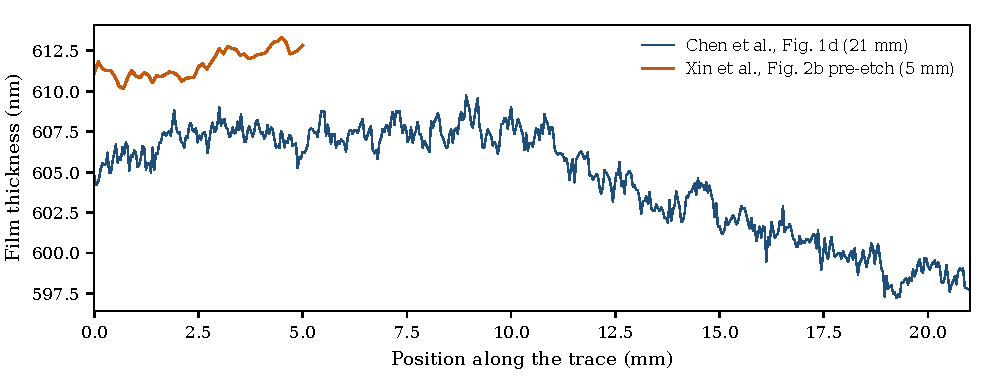
\includegraphics[width=\columnwidth]{fig_thickness.pdf}
\caption{Film thickness used as input.
Chen \emph{et al.}, Fig.~1d, digitized from the vector path \cite{Chen2024}.
Xin \emph{et al.}, Fig.~2b, pre-etch thickness, raster-digitized \cite{Xin2025}.
These are published measurements, not a generated roughness model.}
\label{fig:thick}
\end{figure}

With the Chen trace inserted and no compensation, the intensity-only purity over the available windows is 0.80--0.98 at 2~mm, 0.72--0.89 at 3~mm, 0.38--0.82 at 5~mm, and 0.30--0.66 at 7~mm (Fig.~\ref{fig:kutt}a).
Kuttner's phase-matching-function estimates are 98.0\% and 98.3\%, and the joint-spectral-intensity purities are 95.2\% and 93.8\% \cite{Kuttner2026}.
A 4--7~mm device on this trace does not produce 0.98.
Shortening the device into the 2~mm range is not available as an explanation: both the pump bandwidth and the chip photograph put the length in the 4--7~mm interval.
The phase-matching band points the same way as the measurement once the pump is TM, and the thickness sensitivity is the one checked against the second-harmonic literature at the 10\% level.
The remaining explanation that fits is that their film is smoother than the Chen trace.

\begin{figure}[t]
\centering
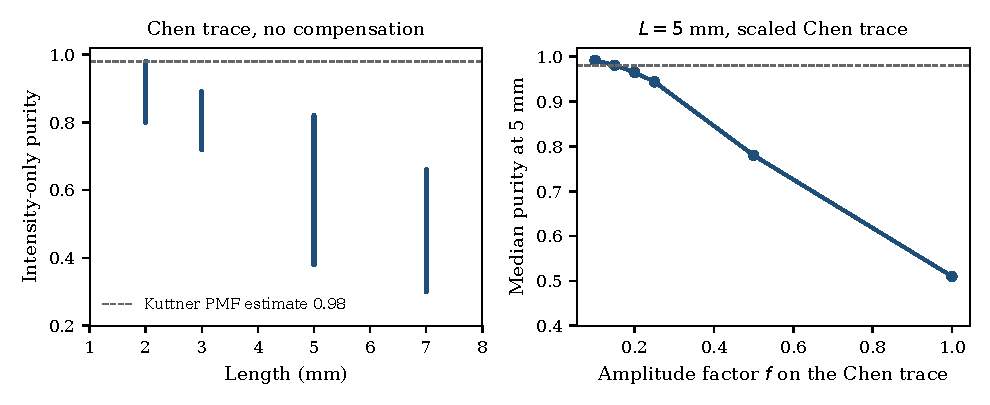
\includegraphics[width=\columnwidth]{fig_kuttner.pdf}
\caption{Uncompensated purity on the Chen trace, TM pump, intensity-only estimator.
(a)~Range over the windows that fit in the 21~mm trace.
The dashed line is the 0.98 phase-matching-function estimate of Kuttner \emph{et al.}
(b)~Median purity at 5~mm when the Chen amplitude is multiplied by $f$.
$f=0.15$ is the largest factor in the scan that still sits at 0.98.}
\label{fig:kutt}
\end{figure}

Scaling the Chen amplitude by a factor $f$ at fixed length 5~mm gives median purities 0.992, 0.981, 0.965, 0.944, 0.780, and 0.51 at $f=0.10$, 0.15, 0.20, 0.25, 0.50, and 1 (Fig.~\ref{fig:kutt}b).
A median of 0.98 therefore needs $f\approx 1/7$.
The 5~mm windows of the Chen trace have RMS 0.64--1.81~nm, so one seventh of that amplitude is an RMS of about 0.1--0.3~nm.
Xin's 5~mm waveguide, RMS 0.82~nm, sits in the same class as Chen's windows, not in the class this estimate assigns to Kuttner.
Kuttner's chip has no published thickness trace, so 0.1--0.3~nm is an inference, not a measurement of that chip.
It becomes a measurement only if that trace is released.

The sentence ``5~mm, uncompensated, purity about 0.5'' is easy to over-read.
It is the median on these two traces: 0.51 when the Chen amplitude is used at full scale in the scaling scan, and 0.509 in the Monte Carlo of the next section.
It is not a property of TFLN films in general.
A film as smooth as the $f\approx 1/7$ case gives a median of 0.98 on the same model.
Adapted poling, on this evidence, does not repair Kuttner's present device.
They already say the compensation is how one would make the phase-matched section longer.
The design use is the one they point at: a wafer that looks like Chen's or Xin's, brought up to the purity of a smooth wafer, and a smooth wafer pushed to a longer device.

\section{Adapted poling, length, and coincidence rate}
\label{sec:adapt}
Adapted poling here means the local grating period follows a measured thickness profile, on a stated pitch, with a stated measurement error added as white noise.
The numbers in this section are medians over 16 Monte Carlo draws at each length, with the 10th and 90th percentiles in brackets.
Ideal purities are an upper bound, not the operating point.
For lengths up to 5~mm the draws are split evenly between the Chen and Xin traces.
At 20~mm only one Chen window exists, so the spread there is the spread of measurement error, chirp, and width noise, not of wafers.
At 15~mm the number of windows is also small.

The thickness sensitivity in these draws is $-3.161$~rad/mm/nm.
It is the TM-pump difference quotient between 560 and 640~nm, an average slope over that 80~nm, not the local derivative at 600~nm.
The previous scan used $-3.687$~rad/mm/nm, the TE-pump central difference at $\pm 10$~nm, and is kept only as a comparison.
Only the thickness term was changed.
The group-velocity ratio and the poling period are still the TE-pump values, as are the width and etch phase coefficients.
If the device is confirmed to use a TM pump, the group-velocity ratio and the poling period have to be recomputed; that is a separate calculation and is not folded into the numbers below.
The loss model is unchanged: propagation loss $-0.54$~dB/cm, facet transmission 0.200, and detection efficiency 68\%.

\begin{figure}[t]
\centering
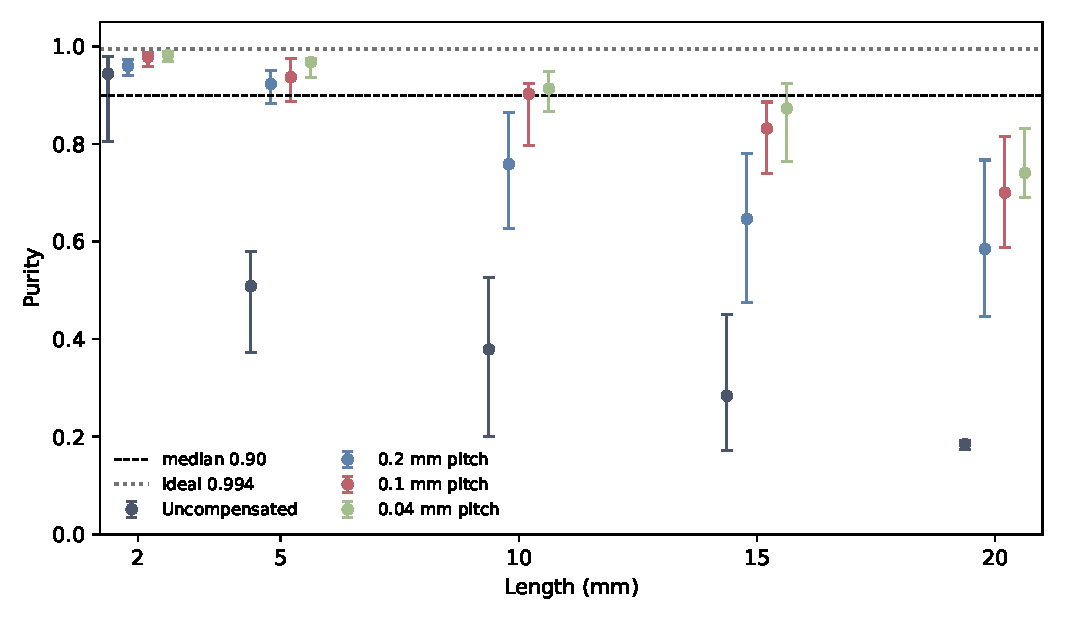
\includegraphics[width=\columnwidth]{fig_mc.pdf}
\caption{Monte Carlo purity against length, 16 draws per length.
Markers are medians; bars run from the 10th to the 90th percentile.
Labels are the measurement pitch and the RMS measurement error.
The dotted line is the ideal upper bound in this run, 0.994 at each length.
The dashed line is the 0.90 median used in the length comparison.
At 15 and 20~mm the percentiles are not a wafer distribution; see the text.
The plotted medians are the $-3.161$~rad/mm/nm rerun.}
\label{fig:mc}
\end{figure}

\begin{table}[t]
\centering
\setlength{\tabcolsep}{2.2pt}
\footnotesize
\caption{Purity versus length, rerun at $-3.161$~rad/mm/nm.
Each entry is the median and the 10th--90th percentile over 16 draws.
Purity does not depend on loss.
Heralding efficiency and coincidence rate are in Table~\ref{tab:rate}, not here.
The 0.5~nm measurement-error column of the previous scan was not repeated and is not shown.
The 0.04~mm pitch is assumed.
Ideal purities in this run round to 0.994 at every length.}
\label{tab:mc}
\small
\begin{tabular}{lccccc}
\toprule
$L$ (mm) & Ideal & None & 0.2~mm, 0.3~nm & 0.1~mm, 0.3~nm & 0.04~mm, 0.3~nm \\
\midrule
2  & 0.994 & 0.944 [0.80--0.98] & 0.960 [0.94--0.97] & 0.978 [0.96--0.99] & 0.982 [0.97--0.99] \\
5  & 0.994 & 0.509 [0.37--0.58] & 0.923 [0.88--0.95] & 0.937 [0.89--0.98] & 0.967 [0.94--0.98] \\
10 & 0.994 & 0.379 [0.20--0.53] & 0.759 [0.63--0.86] & 0.903 [0.80--0.92] & 0.913 [0.87--0.95] \\
15 & 0.994 & 0.284 [0.17--0.45] & 0.646 [0.48--0.78] & 0.832 [0.74--0.89] & 0.873 [0.76--0.92] \\
20 & 0.994 & 0.185 [0.17--0.19] & 0.585 [0.45--0.77] & 0.700 [0.59--0.82] & 0.741 [0.69--0.83] \\
\bottomrule
\end{tabular}
\end{table}

Table~\ref{tab:mc} and Fig.~\ref{fig:mc} are the purity result.
At 5~mm, no compensation gives a median of 0.509.
Measuring every 0.2~mm with 0.3~nm error raises that median to 0.923 (10th--90th percentile 0.88--0.95).
Measuring every 0.1~mm gives 0.937, and every 0.04~mm gives 0.967.
At 10~mm the 0.1~mm pitch has a median of 0.903, with percentile 0.80--0.92.
The median only just clears 0.90, and the 10th percentile is 0.80, so this length does not stay above 0.90.
The 0.04~mm pitch at 10~mm gives 0.913 (0.87--0.95).
The 0.5~nm measurement-error case was not repeated in this rerun.
Loss does not change these purities.
What it changes is the heralding efficiency and the coincidence rate.
The main loss model is taken from the supplemental material of Zhao \emph{et al.}\ \cite{Zhao2020} and is not a random draw: propagation loss $-0.54$~dB/cm near 1569~nm, facet transmission 0.200 ($-7$~dB per facet), and detection efficiency 68\%.
The facets in that measurement were unpolished and unoptimized, so a transmission of 0.200 is a conservative case, not an intrinsic limit of a polished facet.
Pump propagation loss is not included in the main case.
The heralding efficiency is fixed by that formula, with no distribution.
It is 0.134, 0.132, 0.128, 0.124, and 0.120 at 2, 5, 10, 15, and 20~mm (Table~\ref{tab:rate}).
Transmission barely moves with length.
Purity, not transmission, is what fails first.

\begin{table}[t]
\centering
\caption{Main-case heralding efficiency and relative coincidence rate, rerun at $-3.161$~rad/mm/nm.
Propagation loss $-0.54$~dB/cm near 1569~nm, facet transmission 0.200, detection efficiency 68\%, and no pump propagation loss \cite{Zhao2020}.
The heralding efficiency does not depend on the poling or on the thickness coefficient.
Coincidence rates are medians at fixed pump-pulse energy; the absolute scale is set by this loss model and is not a measured brightness.
The 0.04~mm pitch is assumed.}
\label{tab:rate}
\begin{tabular}{lccccc}
\toprule
$L$ (mm) & $\eta_{h}$ & Uncompensated & 0.2~mm & 0.1~mm & 0.04~mm \\
\midrule
2  & 0.134 & 0.143 & 0.143 & 0.143 & 0.143 \\
5  & 0.132 & 0.344 & 0.344 & 0.344 & 0.344 \\
10 & 0.128 & 0.597 & 0.643 & 0.645 & 0.646 \\
15 & 0.124 & 0.541 & 0.900 & 0.907 & 0.911 \\
20 & 0.120 & 0.241 & 1.120 & 1.135 & 1.141 \\
\bottomrule
\end{tabular}
\end{table}

The rate comparison uses the relative coincidence rate in Table~\ref{tab:rate}.
Read at a median purity of at least 0.90:
\begin{itemize}
\item no compensation: only 2~mm qualifies, median purity 0.944, relative rate 0.143, and this is the reference;
\item measure every 0.2~mm: 5~mm, median purity 0.923 (10th--90th percentile 0.88--0.95), relative rate 0.344, which is 2.4 times the uncompensated 2~mm device.
The 10th percentile is 0.88, so this point is also tight;
\item measure every 0.1~mm: 10~mm, median purity 0.903 (percentile 0.80--0.92), relative rate 0.645, which is 4.5 times.
The median only just clears 0.90 and the 10th percentile is 0.80, so the purity does not stay above 0.90.
Under the previous coefficient $-3.687$~rad/mm/nm the same pitch reached only 5~mm, median purity 0.944, 2.4 times; that result is a comparison, not the design point;
\item measure every 0.04~mm: still 10~mm, median purity 0.913 (percentile 0.87--0.95), relative rate 0.646, which is 4.5 times.
\end{itemize}
The 0.04~mm pitch and the 0.3~nm measurement error are both assumed.
The factor is a relative rate on this model, not a measured brightness.

\begin{figure}[t]
\centering
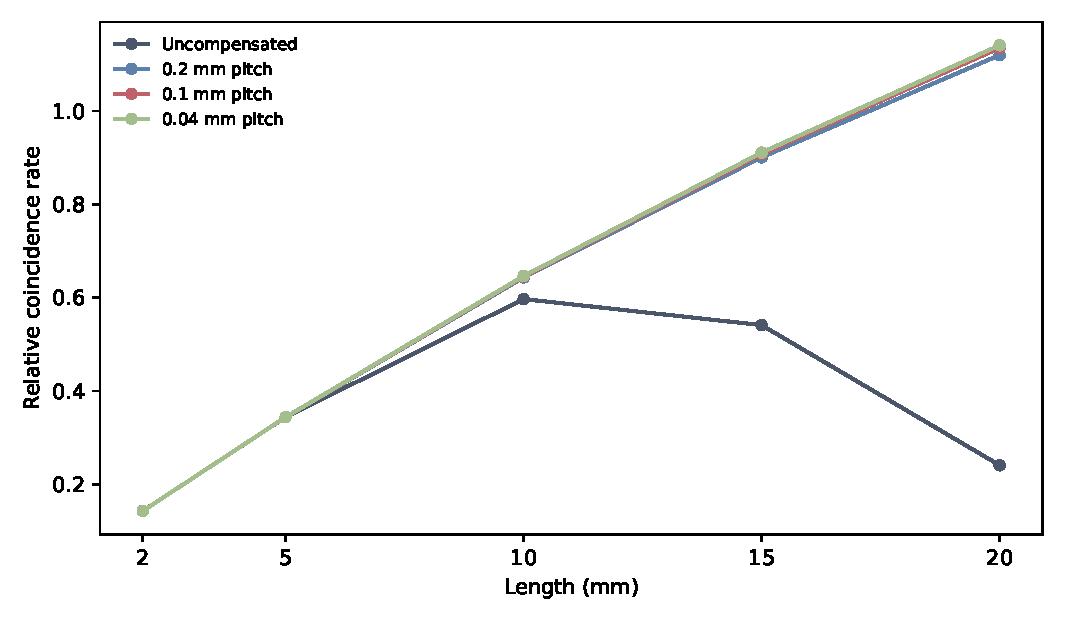
\includegraphics[width=\columnwidth]{fig_yield.pdf}
\caption{Median relative coincidence rate at fixed pump-pulse energy, from the $-3.161$~rad/mm/nm rerun.
The vertical scale is the same as Table~\ref{tab:rate}.
The yield multiples quoted in the text are the main-loss case.
The 0.04~mm curve uses an assumed pitch.}
\label{fig:yield}
\end{figure}

The loss model of the previous draft (0.3~dB/cm, facet transmission 0.5, detection efficiency 0.8) is kept only as an optimistic upper bound on the heralding efficiency.
That efficiency does not depend on the thickness coefficient.
It remains about three times the main case: 0.397 at 2~mm, and 0.393, 0.387, 0.380, and 0.374 at 5, 10, 15, and 20~mm.
The yield multiples under this optimistic bound were not recomputed after the coefficient change.
The multiples quoted above are the main-loss case only.

A separate case that adds the pump propagation loss of $-3.21$~dB/cm near 785~nm, from the same supplemental material, was not repeated at $-3.161$~rad/mm/nm.
It is not part of the result above, and the earlier numerical multiples from that case are not reused.
The term reduces the generation rate, not only the collection, and it grows with length.

\section{What the purity is sensitive to}
\label{sec:sens}
The one-at-a-time scan in this section was not repeated at $-3.161$~rad/mm/nm.
It is the previous scan, at $-3.687$~rad/mm/nm, and it is not a main result.
At 5~mm and a pitch of 0.1~mm, each sensitivity point is 12 draws.
The statistical error on the median is about $\pm 0.03$, which is why the chirp column is not monotonic.
The medians from that previous scan are:
\begin{itemize}
\item residual chirp $0$, $0.25$, $0.5$, $1.0\,\tau^{2}$: purity 0.95, 0.90, 0.92, 0.88, with the 10th--90th percentile at the last point equal to 0.74--0.94;
\item width noise 0, 2, 5, 10~nm: 0.95, 0.93, 0.88, 0.57;
\item measurement error 0.3, 0.5, 1.0~nm: 0.93, 0.87, 0.70.
\end{itemize}
Width noise above 5~nm and a measurement error above 0.5~nm removed most of the adapted-poling gain in that scan.
Both of those inputs are assumed.
The new length comparison, a median of 0.903 at 10~mm with a 0.1~mm pitch, still has to carry that warning: in the previous scan the median fell to 0.57 at a width noise of 10~nm and to 0.70 at a thickness error of 1~nm.
Those two checks have not been recomputed at the new coefficient.

\section{Limits that belong in the result}
\label{sec:limits}
Five restrictions apply to every number above.
They are not footnotes on a result that is otherwise general.

\begin{enumerate}
\item Kuttner's length, width, and etch depth are not given in the original paper or its supplement.
The length interval 4--7~mm is inferred from the pump bandwidth, with a photograph that only supports ``a few millimetres.''
The width, about 0.9~\textmu m with a reading error of about $\pm 0.2$~\textmu m, is read from a micrograph, and the model uses 1.0~\textmu m.
The etch depth of 300~nm is an assumption.
\item ``Five millimetres, uncompensated, purity about 0.5'' holds for thickness variations of the size reported by Chen \emph{et al.}\ and Xin \emph{et al.}
It does not hold for an arbitrary wafer.
The same model gives a median of 0.98 at 5~mm when that amplitude is reduced by about a factor of seven.
\item The width noise (main value 2~nm RMS) and the film-thickness measurement error (main value 0.3~nm) are assumed.
Section~\ref{sec:sens} shows that the adapted-poling gain does not survive a width noise of 10~nm or a measurement error of 1~nm.
The 0.04~mm pitch, which also reaches 10~mm, is assumed.
The 0.1~mm pitch reaches a 10~mm median of 0.903, but the 10th percentile is 0.80, so that length does not stay above 0.90.
The group-velocity ratio and the poling period in the Monte Carlo are still the TE-pump values; the thickness coefficient is the only term that has been updated.
\item There is no experiment in this work.
Every purity, rate, and sensitivity is a simulation on published thickness traces.
The 0.1--0.3~nm figure is an inference about the film that would reconcile the model with Kuttner's purity.
It is not a measurement of their chip.
\item Adapted poling, and the statement that fabrication error limits the useful length, have both been discussed before.
Santandrea \emph{et al.}\ gave the length limit for titanium-diffused waveguides and did not compute a TFLN heralded purity \cite{Santandrea2019}.
Babel \emph{et al.}\ suggested adapted poling, citing Chen \emph{et al.}, or a width adjustment, citing He \emph{et al.}, and did not compute the purity either \cite{Babel2025,He2024}.
The calculation in this paper is the purity, not the first mention of the remedy.
\end{enumerate}

\section{Conclusion}
On a film as uneven as the published Chen and Xin traces, a 5~mm type-II TFLN source does not, in this model, reach the purity Kuttner \emph{et al.}\ report.
The gap closes if the thickness fluctuations are about seven times smaller.
Adapted poling does not change that statement about a smooth wafer.
It changes what can be built on a rough one.
The Monte Carlo uses the TM-pump thickness sensitivity $-3.161$~rad/mm/nm, the difference quotient between 560 and 640~nm and an average slope over that 80~nm, not the local derivative at 600~nm.
The group-velocity ratio and the poling period are still the TE-pump values.
If the device is confirmed to use a TM pump, those two have to be recomputed before the numbers are treated as a device design.
Uncompensated, a median purity of 0.90 is reached only at 2~mm (0.944), with relative coincidence rate 0.143.
Measuring every 0.2~mm reaches 5~mm (median 0.923, 10th--90th percentile 0.88--0.95), 2.4 times that rate.
Measuring every 0.1~mm reaches 10~mm (median 0.903, percentile 0.80--0.92), 4.5 times.
The median only just clears 0.90 and the 10th percentile is 0.80, so this length does not stay above 0.90.
Measuring every 0.04~mm, an assumed pitch, also reaches 10~mm (median 0.913, percentile 0.87--0.95), 4.5 times.
Under the previous coefficient $-3.687$~rad/mm/nm, the 0.1~mm pitch reached only 5~mm at a median purity of 0.944, 2.4 times; that scan is only a comparison.
Those rates use the measured collection loss of Zhao \emph{et al.}: $-0.54$~dB/cm near 1569~nm, facet transmission 0.200 on unpolished and unoptimized facets (a conservative case, not an intrinsic device limit), and detection efficiency 68\%, with no pump propagation loss.
The heralding efficiency is 0.134 at 2~mm and 0.120 at 20~mm.
The optimistic model (0.3~dB/cm, transmission 0.5, detection 0.8) is only an upper bound: about three times the heralding efficiency (0.397 at 2~mm).
The separate pump-loss case at $-3.21$~dB/cm was not repeated at the new coefficient, so its earlier multiples are not reused; that term would reduce the generation rate, not only the collection.
Those gains sit on assumed values for the width noise and the metrology error.
A design that depends on them needs the width variation and the ellipsometer error measured on the same film the poling will track, and it needs the group velocity and the poling period recomputed for a TM pump.
Until then the result is a design bound, not a device performance.
The natural venue is a design paper in \emph{Optics Express} or \emph{Optics Letters}.
A table-top test of the chirp half of the model is possible on bulk material; the thickness half waits on a TFLN chip.

\bibliographystyle{unsrtnat}
\bibliography{refs}

\end{document}
